% Ergebnisse.tex
\chapter{Ergebnisse}

% Ist-Architektur.tex
\section{Ist-Architektur}

% Status: Erstkorrektur
%%%%%%%%%%%%%%%%
%%% Workshop %%%
%%%%%%%%%%%%%%%%
\subsection{Ergebnis des Workshops zur Ist-Architektur}

\subsubsection{Positives und Erhaltenwertes}
Als positiv wurde hervorgehoben, dass die Architektur, zumindest soweit bekannt, nicht an unlösbaren Problemen leidet. 
Dies war in einer früheren Implementation des FreeDesign-Editors der Fall gewesen.

Auch Anforderungsänderung und Erweiterungen konnten bisher problemlos umgesetzt werden.

Die Nutzung von Redux als zentrale Zustandsverwaltung, sowie das Verbinden des Redux-States an die React-Komponenten über \emph{Container}-Objekte wurde ebenfalls als positiv gewertet. 

Als unbedingt erhaltenswerte wurde auch die strikte Trennung zwischen Produktdarstellung und Designdarstellung, sowie den grafischen Komponenten zur Bearbeitung des Designs bewertet. 

%Die grundlegende Strukturierung des Quelltextes innerhalb der Ordner hat sich ebenfalls bewährt und scheint den Einstieg in das Projekt zu fördern. 
%Mitgliedern des Entwicklerteam ist die Strukturierung auch aus andere Projekte bekannt.

\subsubsection{Schwächen und Probleme}
\paragraph{Die unzureichende Strukturierung der Geschäftslogik}
wurde als schwerwiegendste Schwäche der Architektur kritisiert.
Diese ist an verschiedensten Stellen im Quelltext implementiert. Den Mitgliedern des Teams ist oft während der Entwicklungsarbeit nicht klar, ob eine bestimmte Funktionalität bereits implementiert ist und an welcher Stelle im Quelltext diese zu finden ist. 
Daher wird vermutet, dass einige Funktionalitäten mehrfach implementiert sind. 
Dies verstößt gegen das, durch Dave Thomas und Andy Hunt formulierte Prinzip, \emph{"Don’t Repeat Yourself" (DRY)}. Es besagt, dass jedes Wissen innerhalb eines Systems ein einzige, eindeutige und verbindliche Darstellung haben muss \autocite[vgl.][30 - 31]{ThomasAndHunt2020}. 

Quelltext-Duplikate sind aus mehreren Gründen problematisch. Bei Änderungen, müssen mehrerer Stellen im Quelltext angepasst werden. Neben den Funktionalitäten sind auch Unit-Tests mehrfach implementiert, die das Selbe testen und bei Änderungen angepasst werden müssen. Neben dem höheren Entwicklung- und Wartungsaufwand, führen Duplikate auch zu einer größeren JavaScript-Datei für den FreeDesign-Editor. 

\paragraph{Der Mangel inhaltlicher Konventionen} war ein weiterer Kritikpunkt gewesen. Es bestehen technische Konventionen für die Implementation von Quelltext, jedoch mangelt es an fachlichen und inhaltlichen Konventionen. Die Konventionen die in der Ist-Architektur bestehen, resultieren aus der Verwendung von TypeScript, ReactJS und Redux. Beispiele hierfür sind, dass React-Komponenten keine Geschäftslogik enthalten und die Verwendung von \emph{Container}-Objekten zum Verbinden von \emph{React}-Komponenten und \emph{Redux}.
Diese Konventionen wurden jedoch nicht schriftlich festgellegt, sonden bestehen aus mündlichen Absprachen. 
% Darüberhinaus wurden keine Konventionen für den fachlichen und strukturellen Inhalt des Quelltextes festgellegt. 
% Das führt unter anderem dazu, dass es kein Schema für die Bezeichnung von Klassen, Funktionen oder Modulen gibt. Weiterhin werden Funktionen teilweise in Klassen und teilweise in Modulen zusammen gefasst. 

\paragraph{Die Strukturierung der Kommandozeilenprogramme} für die Integration der Designvorlagen wurde ebenfalls kritisiert, welche innerhalb des Editor-Projekt implementiert sind.
Es fällt den Teammitgliedern  schwer, bei Quelltextkomponenten die von den Kommandozeilenprogramme genutzt werden, zu unterscheiden, ob diese exklusiv für die Kommandozeilenprogramme bestehen oder nicht. Dadurch besteht die Gefahr, dass Änderungen der Kommandozeilenprogramme unbeabsichtigt den FreeDesign-Editor mit ändern. Dies verlangsamt die Entwicklungsarbeit und erhöht den Testaufwand.

Die TypeScript-Datei \lstinline|draftImporterCli.ts| welche das Kommandozeilenprogramme zur Konvertierung der Adobe-Illustrator-Dateien enthält, liegt innerhalb des Ordners \lstinline|src|. Für das Kommandozeilenprogramme zum Konvertieren der FreeDesign-Designstruktur in SVG-Dateien ist die Datei \lstinline|designToSvgConverter.ts| im Ordner \lstinline|src/designToSvgCLI| verantwortlich. Diese Strukturierung der Programme wurde als inkonsistent empfunden. 
Es wurde durch das Team angeregt, innerhalb des \lstinline|src|-Ordner einen Ordner ein für Kommandozeilenprogramme zu etablieren, in dem die beiden Programme enthalten sind. Desweiteren wurde vorgeschlagen, dass diese Ordner sämtlichen Quelltextkomponenten enthalten, die exklusiv durch die Kommandozeilenprogramme genutzt werden.  

\paragraph{Das Verwenden generischer Ordner}, welche in Listing \ref{list:genericdirs} angeben sind, wurde durch das Team bemängelt und führt oft zu Unklarheiten. Für die \lstinline|common|-Ordner bestand kein klarer Grund dafür, dass diese zusätzlichen Ebenen geschaffen wurden. Es bestand nur die diffuse Idee, häufig genutzte Komponenten in diesen Ordnern zu sammeln. 

\begin{lstlisting}[language={sh}, label=list:genericdirs, caption=generische Ordner die innerhalb des FreeDesign-Projektes genutzt werden]
src/actions/helper
src/components/common
src/containers/common
src/core/common
src/core/helpers
src/utils
\end{lstlisting}

Carola Lilienthal empfiehlt das Vermeiden von generischen Hilfklassen, da sie von überall her benutzt werden können und die Zusammenarbeit mit anderen Klassen nicht einschränkt wird \autocite[vgl.][159]{Lilienthal2019}. 

Die selben Argumentation liese sich auch das Verwenden generischer Ordnername anwenden. 
% Mit der selben Begründung sollte auch das Verwenden von Ordnern wie \emph{helper}, \emph{common} oder \emph{utils} vermieden werden. Diese Ordner dienen als Sammelorte für Module, deren Zuordnung unklar ist oder für Hilfs-Module. 


% Status: Zweitkorrekt
\subsection{Analyseergebnis der obersten Ordnerebene}
\subsubsection{Übersicht der obersten Ordnerebene}
\label{sec:overview}
Die Quelltextdateien, welche die Anwendungen beschreiben, sind innerhalb des Ordners \lstinline|src| organisiert. 
% Die obersten Ordnerebene des \emph{src}-Ordner spiegelt die Architektur der Anwendung auf höchster Ebene wider.
Abbildung \ref{fig:obersteOrdnerebene} stellt die funktionalen Zusammenhänge der obersten Ordnereben innerhalb des Ordners als Abhängigkeitsgraph dar.  
% Wird innerhalb eines Ordners Quelltext aus einem benachbarten Ordner importiert, wird dies durch eine Pfeilspitze am benachbarten Ordner gekennzeichnet. Beispielsweise importiert Quelltext innherhalb des Ordners \lstinline|designToSvgCLI| Quelltext aus dem Ordner \lstinline|core|.
\begin{figure}[H]
	\centering
    \caption{Übersicht der obersten Ordnerebene innherhalb des Ordner \lstinline|src|}
	\label{fig:obersteOrdnerebene}
	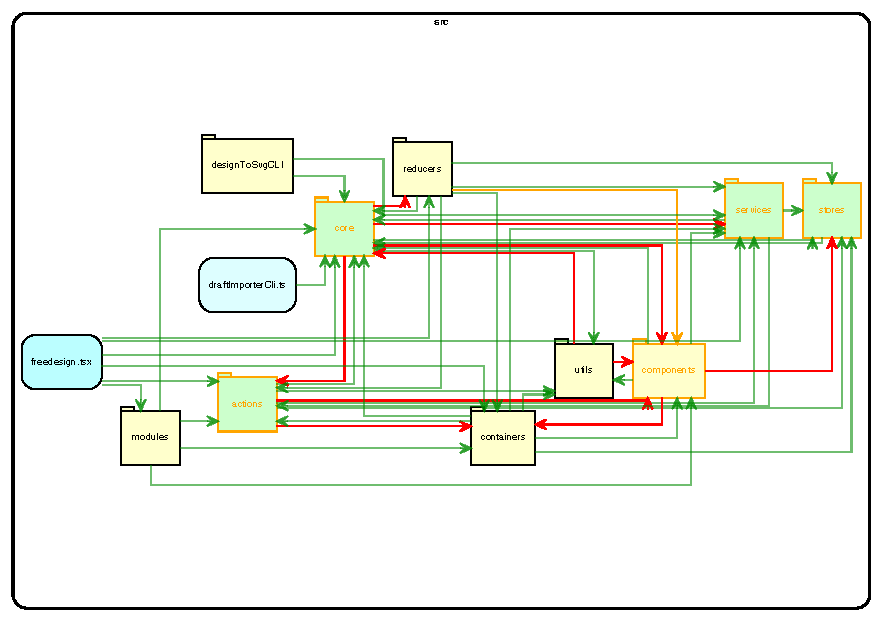
\includegraphics{diagrams/Ist-Architektur/Projektuebersicht.pdf}
\end{figure}


Der Abhängigkeitsgraph zeigt sämtliche Ordner die im Ordner \lstinline|src| enthalten sind, so wie die TypeScript-Dateien \lstinline|freedesign.tsx| und \lstinline|draftImporterCli.tsx|, die ebenfalls im Ordner \lstinline|src| hinterlegt sind.  

Durch die Pfeile werden die Abhängigkeiten der Komponenten gekennzeichnet. Die Pfeilspitze zeigt auf den Ordner, auf dessen Inhalt Zugriffe erfolgen. Beispielsweise greift Quelletext im Ordner \lstinline|designToSvgCLI| auf Quelletext aus dem Ordner \lstinline|core| zu.
Wird eine Abhängigkeit durch das \lstinline|allowed|-Array bestätigt, wird diese durch einen grünen Pfeil dargestellt. Eine Abhängigkeit die durch das \lstinline|forbidden|-Array erfasst wird, wird durch einen roten Pfeil gekennzeichnet. Wird eine Abhängigkeit durch keine der beiden Arrays erfasst, wird diese durch einen orangen Pfeil dargestellt.

Enthält ein Ordner ungenutzten Quelltext, wird dies durch einen orangen Rahmen und einer orangen Bezeichnung gekennzeichnet.

\subsubsection{Ordnerinhalt der obersten Ordnerebene}
\paragraph{Der Ordner \emph{core}} ist für den Anwendungskern vorgesehen und enthält Geschäftslogik sowie grundlegende Funktionalitäten und Datenstrukturen der Anwendung. 
Es ist vorgesehen, dass umgebender Quelletext auf den Quelltext des \lstinline|core|-Ordners zugreifen darf, jedoch ist der Zugriff aus dem \lstinline|core|-Ordner heraus auf den umgebenden Quelletext untersagt. Dem Ordner mangelt es an einer klaren Strukturierung, auf Grund deren die richtige Zuordnung und das Auffinden der Geschäftslogik schwierig sind. 

\paragraph{Im Ordner \emph{components}} sind React-Komponenten zur Erzeugung der grafischen Oberfläche enthalten. Darunter zählen Komponenten zur Erzeugung von Menüs, Dialogen oder auch Werkzeuge zu Designbearbeitung. Die Komponenten besitzen keine Verbindung zum \emph{Redux-State} und rufen keine \emph{Redux-Actions} auf. Die Komponenten können bei der Verwendung mit Eigenschaften versehen werden und damit an Redux gebunden werden. Dadurch ist das Verwenden der React-Komponenten in unterschiedlichen Kontexten möglich.

\paragraph{Der Ordner \emph{containers}} enthält Komponenten (Container-Komponenten), welche die \emph{ReactJS}-Komponenten aus dem Ordner \lstinline|components| mit den \emph{Redux-State} sowie \emph{Redux-Actions} verbindet. Somit verbinden die Container-Komponenten die grafische Oberfläche der Anwendung mit Redux.

% Ein Beispiel hierfür ist der \emph{Container} \lstinline|LoginDialog.tsx|, welcher das Anmeldeformular für die Kundenanmeldung erzeugt. Dieser nutzt Formularelemente und Schaltflächen aus dem \emph{components}-Ordner zur Erzeugung der grafischen Oberfläche. Für die Prüfung, ob der Kunden erfolgreich angemeldet ist, greift der Dialog auf die Kundendaten zu, die im \emph{Redux-State} verwaltet werden. Über eine \emph{Redux-Action} wird die Anmeldung durchgeführt, welche vom \emph{Container} aufgerufen wird. Dadurch das die grafischen Formularelement und Schaltflächen nicht an den Anwendungszustand gebunden sind, konnten sie z.B. auch in einem Dialog zur Kundenregistrierung verwendet werden.


\paragraph{Die Ordner \emph{reducers}, \emph{action} und \emph{stores}} beziehen sich auf Redux und enthalten die Redux-Reducer, die Redux-Actions sowie den Redux-State. Der Redux-States ist auf mehrere Dateien innerhalb des Ordners \lstinline|stores| aufgeteilt. Die Dateien beziehen sich auf unterschiedliche Teile der Anwendung. Beispielsweise wird der Zustand der grafischen Oberfläche in der Datei \lstinline|guiState.ts| verwaltet und der Zustand des Designs, welches gestaltet wird, in der Datei \lstinline|productState.ts| verwaltet. 

\paragraph{Der Ordner \emph{services}} enthält, zusätzlich zu den Redux-Actions \lstinline|ApiActions.ts| im Ordner \lstinline|actions|,  Quelletext zur Kommunikation mit der Unitedprint-API. Außerdem endhält er Quelletext zur Kommunikation mit der Zwischenablage des Betriebssystems, wodurch das Kopieren und Einfügen von Texten beim Bearbeiten eines Designs ermöglicht wird.

% Für die Kommunikation mit der API von Unitedprint wird das Modul \emph{redux-axios-middleware} eingesetzt. 
% Das Module ist eine \emph{Redux}-Middleware für die asynchrone HTTP-Kommunikation. HTTP-Anfragen werden durch den Aufruf von \emph{Redux-Actions} ausgelöst, ebenso werden \emph{Redux-Actions} nach eintreffender Antwort ausgelöst \autocite[vgl.][]{ReduxAxios}. Im Ordner \emph{services} sind die \emph{Redux-Actions} für die API-Aufrufe definiert. Desweiteren enthält der Ordner noch eine Serviceklasse zur Kommunikation mit Zwischenablage des Betriebssystems. Die Klasse ermöglicht das einfügen von Text aus der Zwischenablage in das Design, sowie das Kopier von Text aus dem Design in die Zwischenablage.

\paragraph{Im Ordner utils} befinden sich nur zwei TypeScript-Dateien. Wie bereits im Architektur-Workshop festgestellt, ist die Existenz dieses Ordners fragwürdig und sollte durch die Soll-Architektur aufgelöst werden.  

\paragraph{Der Ordner \emph{modules}} wird ebenfalls durch die Soll-Architektur aufgelöst, da er React- und Redux-Komponenten enthält, welche in die Ordner \lstinline|components| und \lstinline|containers| integriert werden können.

\paragraph{Im Ordner \emph{styles}} sind globalen \emph{CSS}-Definitionen untergebracht, die das optische Erscheinungsbild der Anwendung beschreiben. Die Definitionen werden ausschließlich Komponenten im Ordner \emph{components} verwendet. 

\paragraph{Der Ordner \emph{designToSvgCLI}} enthält das Kommandozeilenprogramm für die Design-SVG-Konvertierung im Integrationsprozess der Designvorlagen, welche im Abschnitt \ref{sect:Integrationsprozess_Designvorlagen} beschrieben wurde.


\paragraph{}Die TypeScript-Datei \lstinline|freedesign.tsx| ist die Startdatei des FreeDesign-Editors, über die das Programm gestartet wird. Für das Kommandozeilen-Programm zum Import der AI-Dateien, welches ebenfalls in Abschnitt \ref{sect:Integrationsprozess_Designvorlagen} beschrieben wurde, ist die Datei \lstinline|draftImporterCli.ts| als Startdatei vorgesehen.


% \paragraph{Zugriffe}
% Die grünen Zugriffspfeile stellen erwartete Zugriffe dar und sind somit gewollte Kopplungen der Einzellkomponenten. Im Gegensatz dazu sind die roten und orangen Zugriffspfeile ungewollte Zugriffe und wurden mit der Zeit integriert. Bei den roten Zugriffen besteht außerdem das Problem, dass diese Zyklen erzeugen und damit gegen die Forderung an eine Architektur, zyklusfrei zu sein, verstoßen. 

% Es bestehe sowohl einzelne Zyklen, wie zwischen den Ordner \emph{core} und \emph{services} sowie Zyklengruppen. Ein Beispiel hierfür ist die Gruppe bestehend aus \emph{actions}, \emph{utils} und \emph{core}.
% Auch innerhalb der Ordner bestehe Zyklen wischen Unterkomponenten. 
% Insgerammt wurden 14 Zyklen festgestellt.

% \paragraph{Verwaister Quelltext}
% Innerhalb der orange gekennzeichneten Ordner befinden sich verwaiste Quelltextabschnitte, welche nicht aufgerufen werden. Solche Quelltextstellen können die Verständlichkeit des Quelltext einschänken. 


% \begin{figure}[H]
% 	\centering
% 	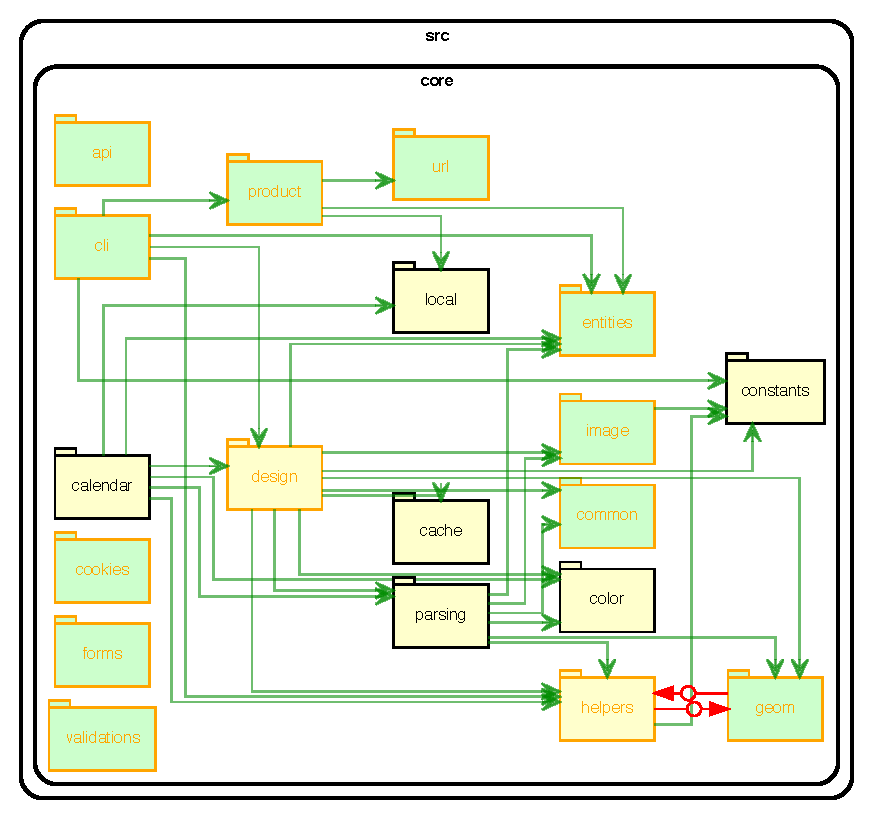
\includegraphics{diagrams/Ist-Architektur/core-graph.pdf}
% 	\caption{Übersicht  }
% 	\label{fig:coreGraph}
% \end{figure}


% Produktdarstellung.tex
\subsection{Produktdarstellung}
Eine zentrale Komponenten der Anwendung ist die Darstellung einer Produktseite, welche auf dem \textit{SVG}-Format basiert.
Das SVG-Format ist eine XML-basiertes Markup-Sprache welche eine zweidimensionale Grafik beschreibt und innherhalb von HTML-Quelltext platziert werden kann \autocite[vgl.][]{AboutSVG}. 

Wie von Abbildung \ref{fig:Produktdarstellung} zu entnehmen ist, werden für das Erzeugen der \textit{SVG}-Struktur \textit{ReactJS}-Komponenten genutzt, die exklusiv für die Produktdarstellung erstellt wurden. Diese Komponenten finden in keinem anderem Zusammenhang Verwendung und sind eng an die Produktdarstellung gekoppelt. 
Zur Darstellung des Produktes gehören das Darstellen von Beschnittlinien, Falzlinien, Nutlinien, Bereichen die nicht bedruckbar sind, sowie Seitenbezeichnungen. Bei einigen Produkten, Textilien oder Werbeprodukte, kann im Hintergrund eine Abbildung des Produktes dargestellt werden. Die Komponente \textit{SVGPageRenderer} ist für verantwortlich für die Produktdarstellung und wird Komponente \textit{PagePresenter.tsx} eingesetzt. Diese wiederum ist für Präsentation des Produktes innerhalb des FreeDesign-Editors verantwortlich und ermöglicht das Rotieren, Skalieren sowie das Verschieben der Darstellung. 


Das Produkt wird durch eine Struktur beschrieben, welche im \textit{core}-Ordner hinterlegt ist. Die Struktur enthält sowohl geometrische Information für die Produktdarstellung, als auch Produktspezifische eigenschaften, wie die Existenz von Beschnittlinien. 

Für die Darstellung innerhalb des FreeDesign-Editors ist die Nutzung von mathematischen Operationen notwendig, die im Anwendungskern definiert sind. 

\begin{figure}[H]
    \centering
    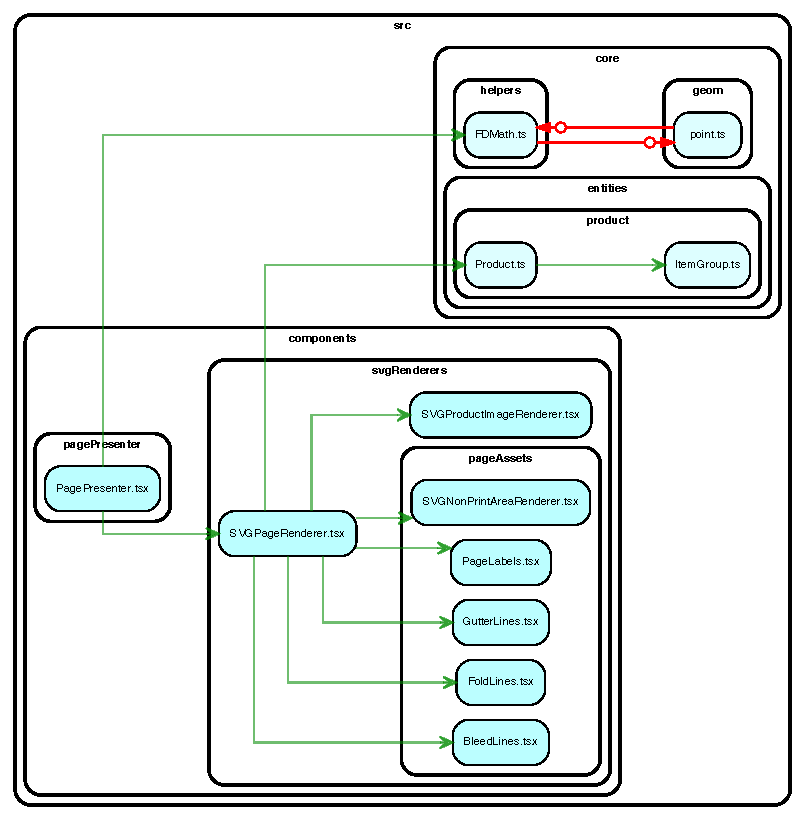
\includegraphics{diagrams/Ist-Architektur/page-presenter-analysis.pdf}
    \caption{Abhängigkeiten der Komponenten für Produktdarstellung}
    \label{fig:Produktdarstellung}
\end{figure}

Der Produktdarstellung kann ein Kindelement übergeben werden, welches in die die Produktdarstellung eingebettet werden. 

\lstinputlisting[frame=single,label=beispielcode,caption=Quelletext-Bsp.: Designdarstellung eingebettet Kindelement]{sourcecode/product.tsx}

\begin{enumerate}
\item{Mathematik}
\item{Produktdarstellung}
\item{Produktstruktur} 
\end{enumerate} 
% Status: Erstkorrektur
% Designdarstellung.tex

\subsection{Designpräsentation}
Die Designpräsentation basiert ebenfalls auf dem SVG-Format, welche durch die React-Komponente \lstinline|DesignPresenter.tsx| erzeugt wird. 

Die Designpräsentation wird der Produktpräsentation als Kindkomponente übergeben. Dadurch sind beiden React-Komponenten voneinander entkoppelt und das Design wird lediglich innerhalb der Produktdarstellung dargestellt.

Die Abbildung \ref{fig:Designdarstellung} weißt die Abhängigkeiten der Designpräsentation auf.

\begin{figure}[H]
    \centering
    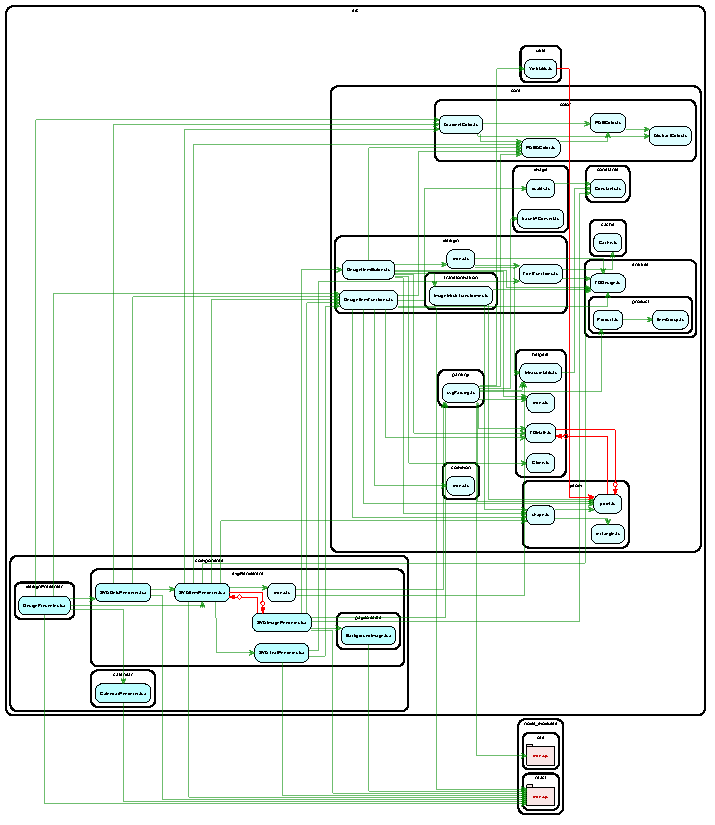
\includegraphics{diagrams/Ist-Architektur/design-presenter-analysis.pdf}
    \caption{Abhängigkeiten der Komponenten für Designdarstellung}
    \label{fig:Designdarstellung}
\end{figure}

Die Designpräsentation ist von einige Datenstrukturen und Funktionalen der \lstinline|core|-Komponente abhängig. 

Folgende Bausteine wurden aus den Abhängigkeiten extrahiert.
\begin{multicols}{2}
\begin{tabular}{ll}
\hline
\textbf{Bildverarbeitung} 
& core/image/* \\
\hline
\textbf{Cache} 
& core/cache/Cache.ts \\
\hline
\textbf{Designdarstellung} 
& components/svgRenderers/* \\
& components/designPresenter/* \\
\hline
\textbf{Designobjekt-Transformation}
& core/design/transformation/*	\\
\hline
\textbf{Designobjekterzeugung} 
& core/design/DesignItemBuilder.ts \\
\hline
\textbf{Designstruktur}
& core/entities/FDDesign.ts \\
\hline
\textbf{Farbstruktur}
& core/color/* \\
\hline
\textbf{JavaScript-Erweiterung} 
& core/helpers/Clone.ts \\
& core/helpers/index.ts \\
\hline
\textbf{Mathematik} 
& core/geom/*	               \\ 
& core/helpers/FDMath.ts	   \\ 
& utils/WebUtils.ts	           \\ 
\hline
\textbf{Maßeinheit-Konverter} 
& core/helpers/MeasureUtils.ts \\
\hline
\textbf{Produktstruktur} 
& core/entities/product/*	\\
\hline
\textbf{Schriftverarbeitung} 
& core/design/FontFunctions.ts \\
\hline
\textbf{SVG-Parser}
& core/parsing/svgParsing.ts \\
\hline
\textbf{XML-Parser}
& utils/WebUtils.ts \\
\end{tabular} 

%  \begin{tabular}{lr}
    % Pfad	                                            &   Komponente \\
    % \hline
    % core/image/*                                    &	Bildverarbeitung  \\
    % core/cache/Cache.ts	                            &   Cache  \\
    % components/svgRenderers/SVGTextRenderer.tsx	    &   Designdarstellung  \\
    % components/svgRenderers/SVGImageRenderer.tsx	&   Designdarstellung  \\
    % components/svgRenderers/SVGItemRenderer.tsx	    &   Designdarstellung  \\
    % components/svgRenderers/SVGDefsRenderer.tsx	    &   Designdarstellung  \\
    % components/svgRenderers/SVGPageRenderer.tsx	    &   Designdarstellung  \\
    % components/svgRenderers/index.ts        	    &   Designdarstellung  \\
    % components/designPresenter/DesignPresenter.tsx	&   Designdarstellung  \\
    % core/design/transformation/*	                &   Designobjekt-Transformation  \\
    % core/design/DesignItemBuilder.ts	            &   Designobjekterzeugung  \\
    % core/entities/FDDesign.ts	                    &   Designstruktur  \\
    % core/color/*	                                &   Farbstruktur  \\
    % core/helpers/Clone.ts	                        &   JavaScript-Erweiterung  \\
    % core/helpers/index.ts	                        &   JavaScript-Erweiterung  \\
    % core/geom/*	                                    &   Mathematik  \\
    % core/helpers/FDMath.ts	                        &   Mathematik  \\
    % utils/WebUtils.ts	                            &   Mathematik  \\
    % core/helpers/MeasureUtils.ts                    &	Maßeinheit-Konverter  \\
    % components/svgRenderers/pageAssets/*	        &   Produktdarstellung  \\
    % components/svgRenderers/SVGProductImageRenderer.tsx	    &   Produktdarstellung  \\
    % core/entities/product/*	                        &   Produktstruktur  \\
    % core/design/FontFunctions.ts	                &   Schriftverarbeitung  \\
    % core/parsing/svgParsing.ts	                    &   SVG-Parser  \\
    % utils/WebUtils.ts	                            &   XML-Parser  \\
%  \end{tabular} 
\end{multicols}
% Designbearbeitung.tex
\subsection{Designbearbeitung}
Die dritte Hauptkomponente des FreeDesign-Editors ist das bearbeiten des Designs. Hierfür stellt der Editor Eingabekomponenten zur Verfügung, welche Änderungen der Designstruktur im \textit{Redux-State} bewirken. Auf diese Änderungen reagiert die Designdarstellung und löst eine Aktualisierung aus, wodurch keine Abhängigkeiten zwischen der Darstellung des Designs und der Bearbeitung des Designs bestehen. Beide Komponenten greifen lediglich auf die selbe Designstruktur zu.  
Die \textit{Container}-Komponente \textit{Stage.tsx} verbindet alle Komponenten, die für die Bearbeitung des Designs Notwendig sind. Hierzu gehören grafisch Komponente zur Darstellung von Auswahlrahmen, eine Texteingabe sowie Hilfswerkzeugen, wie einem Lineal oder einem Gitter. 
Desweiteren ist sie mit dem \textit{Redux-Store} verbunden und ruft sie verschieden \textit{Redux-Actions}. 
Mit  1260 Quelltextzeilen, 51 Funktionen und 46 Importen, handelt es sich um die komplexeste Komponente des FreeDesign-Editor und kann als eine \textit{Man-in-the-middle-Klasse} bezeichnet werden. Hierbei handelt es sich um ein Antimuster bei dem eine Klasse zu viele zuständigkeiten hat \autocite[vgl.][619]{Geirhos2015}.
Im allgemeinen ist der Quelltext und die Abhängigkeiten für die Designbearbeitung sehr komplex und ungenügend strukturiert. Das bearbeiten eines Designs ist die Kernfunktionalität des FreeDesign-Editor und sollte von einer Soll-Architektur aus der restlichen Anwendung als entkoppelte Komponente extrahiert werden. 
% GUI.tex
\subsection{Grafische Oberfläche}
Die grafische Oberfläche bindet den Baustein zum Designbearbeitung und damit auch die Bausteine Design- und Produktdarstellung ein. Um diese Bausteine herum sind verschiedenste grafische Elemente integriert, die das Bearbeiten des Design unterstützen, sowie die Produktkonfiguration. Außerdem sind Elemente zur steuern  und visualisieren von Kundendaten enthalten, wie das Speicher und Öffnen von Designentwürfen oder die Anzeige des Warenkorbs.
Die Abhängigkeiten der grafischen Oberfläche sind sehr komplex und sind in der Darstellung \emph{D3\_Grafische\_Oberfläche.html} visualisiert. 

Die grafische Oberfläche ist auch das volatilste Element des FreeDesign-Editors und unterliegt ständiger Änderungen und Erweiterungen. Basierend auf Martin (\citeyear[119]{Martin2018}) sollte der volatile Teile eines Quelltext von stabilen Teile isoliert werden. Gerade im Quelltext für die Bereitstellung der Funktionalitäten zu Verschieben, Rotieren und Skalieren von Designobjekt besteht die Gefahr, dass Änderungen der Grafischen Darstellung dem stabile Quelltext für Objekt-Transformationen beschädigt. 
Folgende Bausteine der grafischen Oberfläche wurden identifiziert.

\begin{multicols}{2}    
    \begin{enumerate}
    \item API-Kommunikation
    \item Anwender-Menü
    \item Anwenderregistrierung
    \item Bestätigungsdialog
    \item Bild-Upload
    \item Bildmaskeneditor
    \item Bildverarbeitung
    \item Cache
    \item Cookie-Verarbeitung
    \item Design-Parser
    \item Designbearbeitung
    \item Designdarstellung
    \item Designelementauswahl
    \item Designgalerie
    \item Designobjekt-Transformation
    \item Designobjekterzeugung
    \item Designstruktur
    \item Dialogfenster
    \item Farbstruktur
    \item Fehlerdialog
    \item Formularverarbeitung
    \item Fotogalerie
    \item Grafische-Oberfläche
    \item JavaScript-Erweiterung
    \item Kalendariumerzeuger
    \item Kopfleiste
    \item Kurzinformation
    \item Mathematik
    \item Maßeinheit-Konverter
    \item Produktdarstellung
    \item Produktkonfigurator
    \item Produktseiten-Bild-Konverter
    \item Produktstruktur
    \item Referenzwerkzeug
    \item SVG-Parser
    \item Schriftverarbeitung
    \item Speicherkomponente
    \item Startvideo
    \item Tastatur-Kurzbefehle
    \item Textschlüsselsammlung
    \item URL-Verarbeitung
    \item Warenkorb
    \item Werkzeugmenü
    \item XML-Parser
    \item Zwischenablageschnittstelle
\end{enumerate}
\end{multicols}
\subsection{Kommandozeilenprogramm Adobe-Illustrator-Designkonvertierung}

\begin{figure}[H]
    \centering
    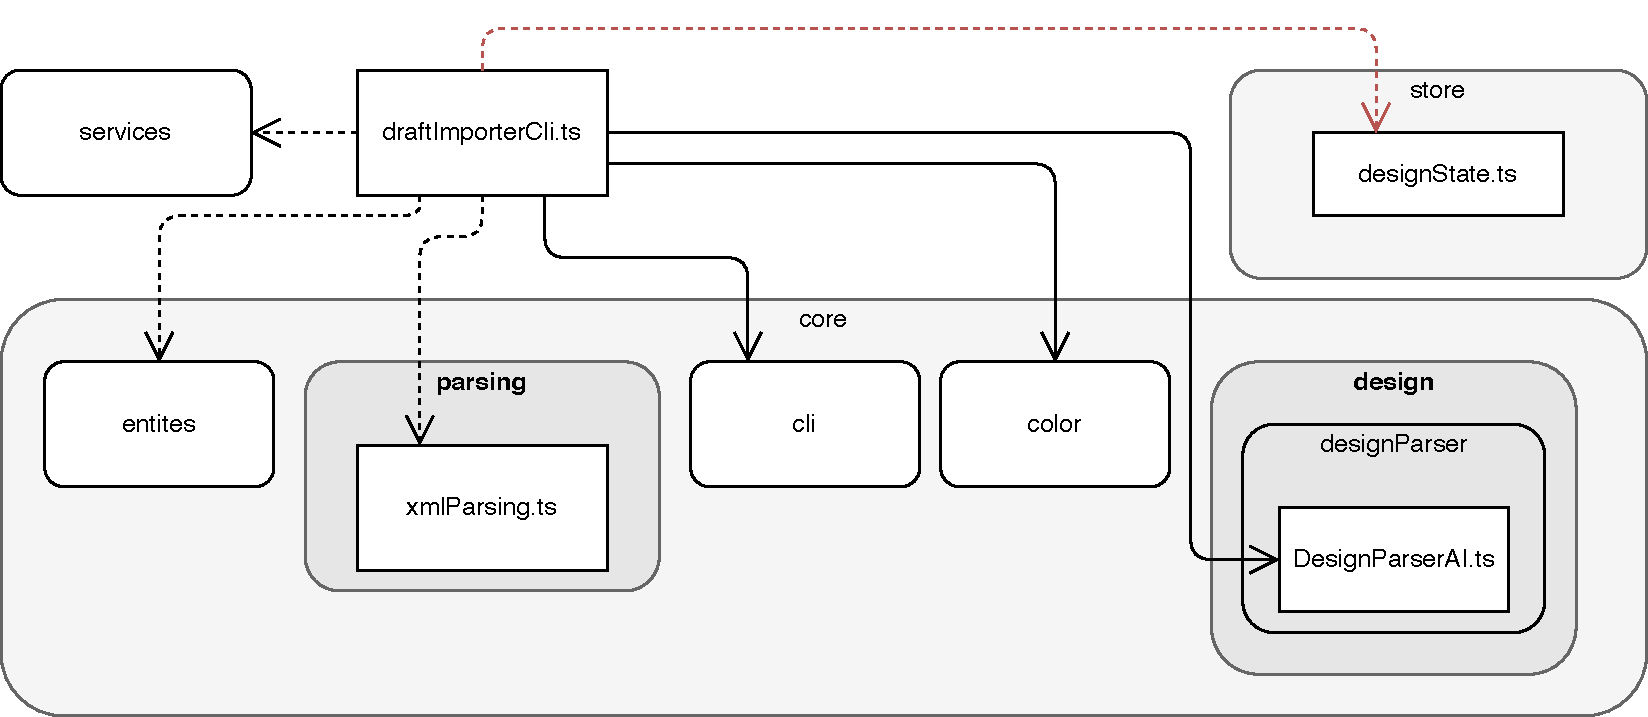
\includegraphics{diagrams/Ist-Architektur/draftImporter-analysis.pdf}
    \caption{Abhängigkeiten der Komponenten für das Kommandozeilenprogramm zur Konvertierung von Designs die mit Adobe-Illustrator erstellt wurden zu FreeDesign-Designs.}
    \label{fig:DesignImport}
\end{figure}

\begin{multicols}{2}    
    \begin{enumerate}
    \item API-Kommunikation
    \item Bildverarbeitung
    \item Cache
    \item Designstruktur
    \item Design-Parser
    \item Produktstruktur
    \item Farbstruktur
    \item JavaScript-Erweiterung
    \item Mathematik
    \item Maßeinheit-Konverter
    \item SVG-Parser
    \item Schriftverarbeitung
    \item XML-Parser
\end{enumerate}
\end{multicols}
\subsection{Kommandozeilenprogramm Design-SVG-Konverter}
Nach der, in Kapitel \ref{Kommandozeilenprogramm Adobe-Illustrator-Designkonvertierung} \emph{Kommandozeilenprogramm Adobe-Illustrator-Designkonvertierung} beschrieben, Konvertierung der Designvorlagen, werden Derivate der Vorlagen erzeugt. Diese enthalten übersetzte Texte, für die unterschiedlichen Sprachen in denen die Vorlagen angeboten werden. Um die Vielfalt der Vorlagen zu erhöhen, werden außerdem weitere Derivate mit unterschiedlichen Farbzuordnung erzeugt. Die Erzeugung der Derivate ist nicht Bestandteil des FreeDesign-Projektes. Jedoch werden in einem letzten Prozessschritt 3D-Vorschaubilder der Derivate zur Präsentation im Webshop erzeugt. Die Erzeugung der Vorschaubilder, die ebenfalls nicht Teil des FreeDesign-Projektes ist, basiert auf SVG-Dateien die durch das FreeDesign-Projektes erzeugt werden. Hier zu 


Konvertierung der Designvorlagen, werden in einem weiteren Prozessschritt 3D-Vorschaubilder für die Präsentation im Webshop erzeugt. 

Das FreeDesign-Projekt unterstützt den, im Kapitel \ref{Kommandozeilenprogramm Adobe-Illustrator-Designkonvertierung} \emph{Kommandozeilenprogramm Adobe-Illustrator-Designkonvertierung} beschrieben, Import der Designvorlagen durch ein weiteres Kommandozeilenprogramm. 

\begin{figure}[H]
    \centering
    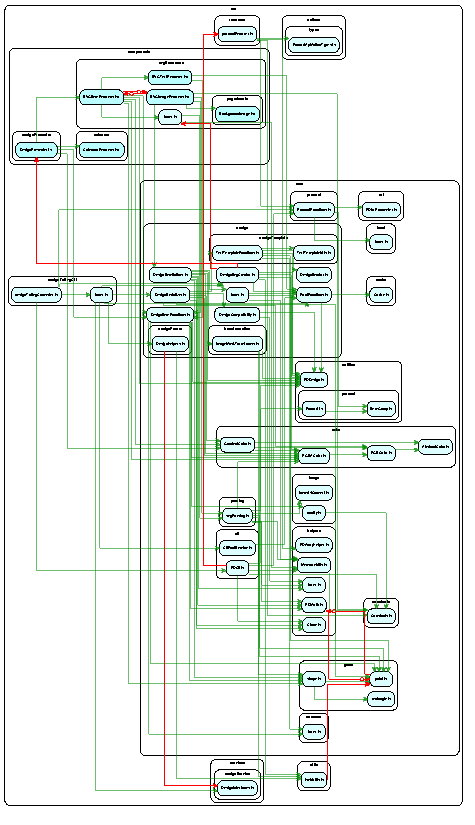
\includegraphics{diagrams/Ist-Architektur/designToSvgCLI-analysis.pdf}
    \caption{Abhängigkeiten der Komponenten für das Kommandozeilenprogramm zur Konvertierung von Designs zu SVG-Dateien.}
    \label{fig:DesignToSvg}
\end{figure}
\begin{multicols}{2}
    \begin{enumerate}
    \item API-Kommunikation
    \item Bildverarbeitung
    \item Cache
    \item Designdarstellung
    \item Design-Parser
    \item Design-Serialisierung
    \item Designstruktur
    \item Farbstruktur
    \item JavaScript-Erweiterung
    \item Mathematik
    \item Maßeinheit-Konverter
    \item Produktstruktur
    \item Schriftverarbeitung
    \item SVG-Parser
    \item Vorlagekonverter
\end{enumerate}

\end{multicols}
\subsection{Zusammenfassung der Ist-Architektur}
% Auf fehlendes SOLID eingehen
% Übersicht der Quelltextzuordnung im Anhang

% Soll-Architektur.tex
\section{Soll-Architektur}
\subsection{nichtfunktionalen Anforderungen}


\subsection{technische Anforderungen}
% \subsection{Anforderungen an die Soll-Architektur} % Softwarearchitektur S. 108 - 

% \subsubsection{Funktionale Anforderungen}
% Die Tabelle \ref{table:fa} beschreibt die funktionalen Anforderungen die das FreeDesign-Projekt bereitstellen muss. Die Anforderungen sind unterteilt in \emph{FreeDesign-Webapp}, \emph{AI-Design-Converter-CLI} sowie \emph{SVG-Page-Renderer-CLI}.
% Der Teil \emph{FreeDesign-Webapp} bezieht auf die Webanwendung des FreeDesign-Editor und ermöglicht somit die Definition weiter grafischer Oberflächen des FreeDesign Editors. Denkbar hierfür wäre eine separate Oberflächen für native\footnote{Dies wäre durch die Nutzung von ReactNative möglich. \url{https://reactnative.dev}} Anwendung die sich an eine mobile Endgeräte richten. 
% \begin{filecontents}[overwrite]{\jobname-fa.tex}
%     \begin{longtable}{r@{\hspace{3mm}}lX}
%     \caption{Auflistung funktionaler Anforderungen}\\
%     \label{table:fa}
%     \rownumbereset
%     & \textbf{Anforderung} & \textbf{Beschreibung} \\
%     \hline
%     \hline
%     \multicolumn{3}{l}{\textbf{FreeDesign-Webapp}} \\
%     \hline
%     \rownumber & Darstellung Produktseite & Die Darstellung einer Produktseite ist abhängig vom Produkt und beinhaltet das Darstellen produktspezifischer Eigenschaften. \\
%     \rownumber & Darstellung Designs & Ein Design wird innerhalb einer ein Produktseite darzustellen. \\
%     \rownumber & Mehrsprachigkeit & Die Texte der grafische Oberfläche müssen für eine gegebene Landesprache übersetzt sein. \\
%     \end{longtable}
% \end{filecontents}
% \LTXtable{\linewidth}{\jobname-fa.tex}

% \subsubsection{Nichtfunktionale Anforderungen}
% \begin{filecontents}[overwrite]{\jobname-nfa.tex}
%     \begin{longtable}{r@{\hspace{3mm}}lX}
%     \caption{Auflistung der nichtfunktionalen Anforderungen}\\
%     \label{table:fa}
%     \rownumbereset
%     & \textbf{Anforderung} & \textbf{Beschreibung} \\
%     \hline
%     \hline
%     \multicolumn{3}{l}{\textbf{FreeDesign-Webapp}} \\
%     \hline
%     \rownumber & Darstellung Produktseite & Die Darstellung einer Produktseite ist abhängig vom Produkt und beinhaltet das Darstellen produktspezifischer Eigenschaften. \\
%     \rownumber & Darstellung Designs & Ein Design wird innerhalb einer ein Produktseite darzustellen. \\
%     \rownumber & Mehrsprachigkeit & Die Texte der grafische Oberfläche müssen für eine gegebene Landesprache übersetzt sein. \\
%     \end{longtable}
% \end{filecontents}
% \LTXtable{\linewidth}{\jobname-nfa.tex}

% Step 1. Anforderungen festlegen


% 
\subsection{Entwurf einer optimierten Soll-Architektur}
Entwurf einer Soll-Architektur, die die Schwächen der Ist-Architektur ausmerzt.

\subsection{Prototyp}
Implementation der Soll-Architektur in einem Prototypen zur Bestätigung der Machbarkeit.

\section{Migrationsstrategie}
\subsection{Migrationsschritte}
Ausarbeitung von Migrationsschritten die zum Erreichen der Soll-Architektur notwendig sind.

\subsection{Priorisierung}
Priorisierung der Migrationsschritte.

\subsection{Migrationsplan}
Erstellung eines Ablaufplans zu Migration.

\subsection{Vorgehensweise für das Refactoring}
Beschreibung einer Vorgehensweise wie das Refactoring für die einzelnen Migrationsschritte vorgenommen werden sollte.
=> Test-Abdeckung, Separieren von Quelltext, etc.
